\documentclass[fleqn, a4paper, 12pt]{article}
\usepackage{amsmath, amssymb, amsthm}
\usepackage{gensymb}
\usepackage{commath}
\usepackage{xcolor}
\usepackage{cancel}
\usepackage{siunitx}
\usepackage{tikz, pgfplots}
	\usetikzlibrary{calc, hobby, patterns, intersections}
\usepackage{graphicx}
\usepackage{hyperref}
\usepackage{datetime}
\usepackage{ulem}
\usepackage{xfrac}
\usepackage{asymptote}
\usepackage{enumerate}
\setcounter{secnumdepth}{4}
\newcommand\numberthis{\addtocounter{equation}{1}\tag{\theequation}}

\newcommand{\AxisRotator}[1][rotate=0]{%
	\tikz [x=0.25cm,y=0.60cm,line width=.2ex,-stealth,#1] \draw (0,0) arc (-150:150:1 and 1);%
}

\theoremstyle{definition}
\newtheorem{example}{Example}
\newtheorem{definition}{Definition}

\theoremstyle{theorem}
\newtheorem{theorem}{Theorem}

\newenvironment{solution}
{\begin{proof}[Solution]\let\qed\relax}
	{\end{proof}}

\newcommand{\curl}{\mathrm{curl\,}}

%\renewcommand{\int_{min}^{max}}{\int\displaylimits_{min}^{max}}

%opening
\title{Lecture 17}
\author{Aakash Jog}
\date{\formatdate{28}{12}{2014}}

\begin{document}

\maketitle
%\setlength{\mathindent}{0pt}

\tableofcontents

\newpage
\section{Moment of Inertia}

\begin{example}
	Find the moment of inertia of a disk of radius $R$ and mass $m$.
\end{example}

\begin{solution}
	\begin{align*}
		\sigma &= \dfrac{m}{\pi R^2}
	\end{align*}
	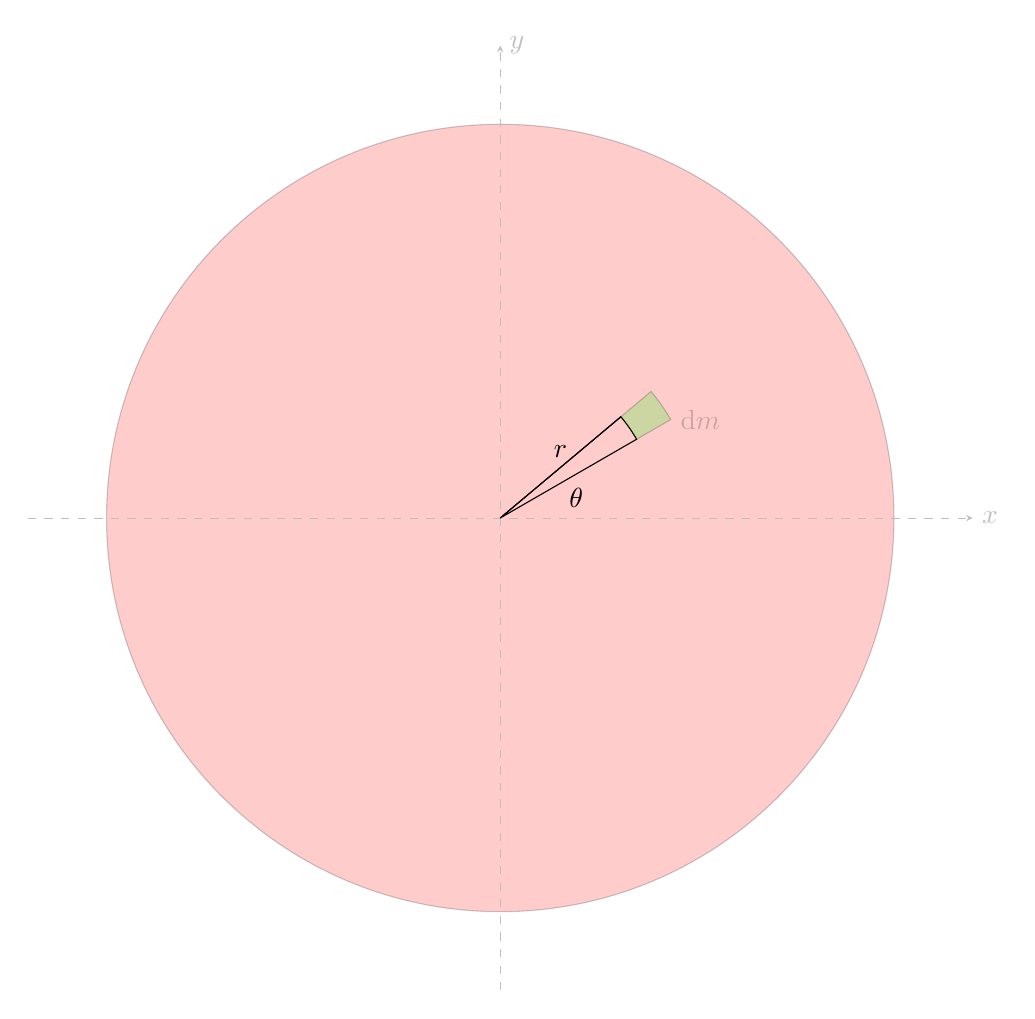
\begin{tikzpicture}
		\filldraw [fill = red, opacity = 0.2] (0,0) circle [radius = 5cm];
		
		\draw [lightgray, ultra thin, dashed, -stealth] (-6,0) -- (6,0) node [right] {$x$};
		\draw [lightgray, ultra thin, dashed, -stealth] (0,-6) -- (0,6) node [right] {$y$};
		
		\draw (30:2) arc (30:40:2cm) -- (0,0) -- cycle;
		\filldraw [fill = green, opacity = 0.2] (30:2.5) arc (30:40:2.5cm) -- (40:2) arc (40:30:2cm) -- cycle node [right] {$\dif m$};
		
		\node at (15:1) {$\theta$};
		
		\draw (0,0) -- (40:2) node [midway, above] {$r$};
	\end{tikzpicture}
	\begin{align*}
		I_z &= \int r^2 \dif m\\
		&= \int\limits_{0}^{R} \int\limits_{0}^{2 \pi} r^2 r \dif \theta \dif r \sigma\\
		&= \sigma \int\limits_{0}^{R} r^3 \dif r \int\limits_{0}^{2 \pi} \dif \theta\\
		&= \sigma \dfrac{R^4}{4} \cdot 2 \pi\\
		&= \dfrac{1}{2} \pi \sigma R^4\\
		&= \dfrac{1}{2} (\pi R^2 \sigma) R^2\\
		&= \dfrac{1}{2} m R^2
	\end{align*}
\end{solution}

\begin{example}
	Find the moment of inertia of a rectangular body.
\end{example}

\begin{solution}
	\begin{align*}
		\sigma &= \dfrac{a b}{m}
	\end{align*}
	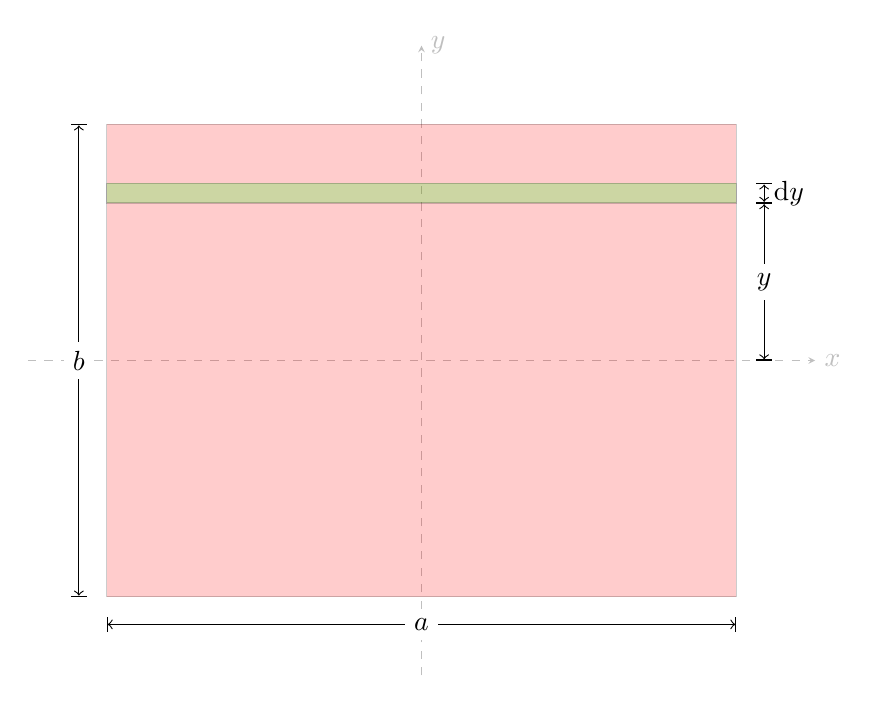
\begin{tikzpicture}
		%definition of origin
		\coordinate (O) at (0,0);
		
		%variables
		\def\a{8};
		\def\b{6};
		
		\def\y{2};
		\def\dy{0.25};
		
		%axes
		\draw [lightgray, ultra thin, dashed, -stealth] ({-(\a/2 + 1)},0) -- ({\a/2 + 1},0) node [right] {$x$};
		\draw [lightgray, ultra thin, dashed, -stealth] (0,{-(\b/2 + 1)}) -- (0,{\b/2 + 1}) node [right] {$y$};
		
		%rectangle
		\filldraw [fill = red, opacity = 0.2] (-\a/2, -\b/2) rectangle (\a/2, \b/2);
		
		%elemental strip
		\filldraw [fill = green, opacity = 0.2] (-\a/2, \y) rectangle (\a/2, \y + \dy);
		
		%dimensions
		\draw [|<->|, yshift = -10] (-\a/2, -\b/2) -- (\a/2, -\b/2) node [midway, fill = white] {$a$};
		\draw [|<->|, xshift = -10] (-\a/2, -\b/2) -- (-\a/2, \b/2) node [midway, fill = white] {$b$};
		
		\draw [|<->|, xshift = 10] (\a/2, 0) -- (\a/2, \y) node [midway, fill = white] {$y$};
		\draw [|<->|, xshift = 10] (\a/2, \y) -- (\a/2, \y + \dy) node [midway, right] {$\dif y$};
	\end{tikzpicture}
	\begin{align*}
		I_x &= \iint y^2 \dif m\\
		&= \int\limits_{-\sfrac{b}{2}}^{\sfrac{b}{2}} y^2 a \dif y \sigma\\
		&= \dfrac{1}{12} a b^3 \sigma\\
		&= \dfrac{1}{12} m b^2
	\end{align*}
	Similarly,
	\begin{align*}
		I_y &= \dfrac{1}{12} m a^2
	\end{align*}
\end{solution}

\begin{example}
	Find the moment of inertia of a sphere
\end{example}

\begin{solution}[Using cylindrical coordinates]
	\begin{align*}
		\rho &= \dfrac{m}{\sfrac{4}{3} \cdot \pi r^3}
	\end{align*}
	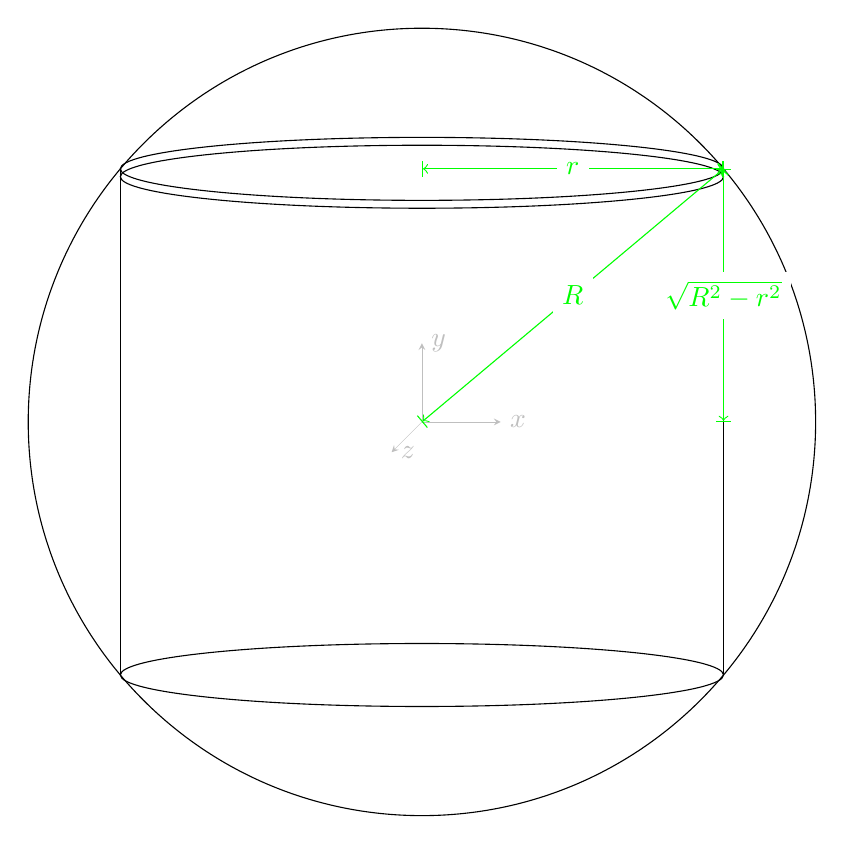
\begin{tikzpicture}
		%variables
		\def\R{5};
		\def\angle{50};

		%axes
		\draw [-stealth, ultra thin, lightgray] (0,0,0) -- (1,0,0) node [right] {$x$};
		\draw [-stealth, ultra thin, lightgray] (0,0,0) -- (0,1,0) node [right] {$y$};
		\draw [-stealth, ultra thin, lightgray] (0,0,0) -- (0,0,1) node [right] {$z$};

		%sphere
		\draw (0,0) circle [radius = \R];

		%cylinder		
		\draw (0, {\R*cos{\angle}}) circle [x radius = {\R*sin{\angle}}, y radius = 0.4];
		\draw (0, {\R*cos{\angle} - 0.1}) circle [x radius = {\R*sin{\angle}}, y radius = 0.4];
		\draw (0, {-\R*cos{\angle}}) circle [x radius = {\R*sin{\angle}}, y radius = 0.4];
		
		\draw ({\R*sin{\angle}}, {\R*cos{\angle}}) -- ({\R*sin{\angle}}, {-\R*cos{\angle}});
		\draw ({-\R*sin{\angle}}, {\R*cos{\angle}}) -- ({-\R*sin{\angle}}, {-\R*cos{\angle}});
		
		%dimensions
		\draw [green, |<->|] (0,0) -- ({\R*sin{\angle}}, {\R*cos{\angle}}) node [midway, fill = white] {$R$};
		
		\draw [green, |<->|] (0, {\R*cos{\angle}}) -- ({\R*sin{\angle}}, {\R*cos{\angle}}) node [midway, fill = white] {$r$};
		
		\draw [green, |<->|] ({\R*sin{\angle}},0) -- ({\R*sin{\angle}}, {\R*cos{\angle}}) node [midway, fill = white] {$\sqrt{R^2 - r^2}$};
	\end{tikzpicture}
	\begin{align*}
		I &= \int\limits_{0}^{R} r^2 \dif m\\
		&= \int\limits_{0}^{R} r^2 \cdot 2 \pi r h \dif r \rho\\
		&= \dfrac{2}{3} m R^2
	\end{align*}
\end{solution}

\begin{solution}[Using spherical coordinates]
	\begin{align*}
		\rho &= \dfrac{m}{\sfrac{4}{3} \cdot \pi R^3}
	\end{align*}
	\begin{align*}
		I &= \int (r')^2 \dif m\\
		&= \int\limits_{0}^{\pi} \int\limits_{0}^{2 \pi} \int\limits_{0}^{R} r^2 \sin^2 \theta \rho r^2 \sin \theta \dif r \dif \varphi \dif \theta\\
		&= 2 \pi \rho \int\limits_{0}^{\pi} \sin^2 \theta \sin \theta \dif \theta \int\limits_{0}^{R} r^4 \dif r\\
		&= \dfrac{2}{5} m R^2
	\end{align*}
\end{solution}

\section{Rigid Body Dynamics}

\begin{example}
	A rope is wound on a cylindrical pulley of mass $m_1$, and a mass $m_2$ is attached to the free end of the rope. The pulley is fixed through its centre. The system is released from rest. Find the acceleration of $m_2$.
\end{example}

\begin{solution}
	\hspace{1cm}\\
	\begin{tikzpicture}
		%definition of origin
		\coordinate (O) at (0,0);
		
		%variables
		\def\R{2};
		\def\l{6};
		
		%coordinates
		\coordinate (rope end) at (\R, -\l);
		
		%
		\draw (O) circle [radius = \R];
		\fill (O) circle [radius = 1pt] node [left] {$m_1$};
		
		\draw ($ (O) + (0:\R) $) -- (rope end);
		
		\fill (rope end) circle [radius = 3 pt] node [right] {$m_2$};
		
		%forces
		\draw [red, -stealth] (O) -- ++(90:1) node [above] {$N$};
		\draw [red, -stealth] (O) -- ++(-90:1) node [below] {$m_1 g$};
		\draw [red, -stealth] ($ (O) + (0:\R) $) -- ++(-90:1) node [right] {$T$};
		
		\draw [blue, -stealth] (rope end) -- ++(90:1) node [right] {$T$};
	\end{tikzpicture}
	\begin{align*}
		N &= m_1 g + T\\
		m_2 g - T &= m_2 a\\
		RT &= \dfrac{1}{2} m_1 R^2 \alpha\\
		&= \dfrac{1}{2} m_1 R^2 \dfrac{a}{R}
	\end{align*}
	Solving,
	\begin{align*}
		a &= \dfrac{m_2 g}{\sfrac{1}{2} \cdot m_1 + m_2}
	\end{align*}
\end{solution}

\subsection{Pure Rolling}

\begin{tikzpicture}
	\def\PI{3.14159265};
	\def\R{3};

	\draw ({-(\R + 1)}, 0) -- ({\R + 1}, 0);

	\draw (0,\R) circle [radius = \R];

	\draw [dashed] (0,0) -- (0,2*\R);
	
	\draw [-stealth] (0,\R) -- ++(0:1) node [right] {$R \omega$};
	\draw [-stealth] (0,2*\R) -- ++(0:2) node [right] {$2 R \omega$};
\end{tikzpicture}

\begin{align*}
	x &= R \theta\\
	\therefore v_{\text{COM}} &= R \omega
\end{align*}
The point of contact is the instantaneous axis of pure rotation.

\begin{align*}
	\overrightarrow{L_0} &= \cancelto{0}{\overrightarrow{r_{\text{COM}}}} \times (m \overrightarrow{v_{\text{COM}}}) + \left( \dfrac{1}{2} m R^2 \omega \right) (-\hat{z})\\
	&= -\dfrac{1}{2} m R^2 \omega \hat{z}
\end{align*}

\begin{example}
	A body is rolling down an inclined plane. Find the acceleration of the body.
\end{example}

\begin{solution}[Using COM axis]
	Friction must exist for the motion to be purely rolling.\\
	\begin{tikzpicture}
		\def\angle{30};
		\def\l{15};
		\def\R{3};
		
		\node at ({180 - (\angle/2)}:1) {$\theta$};
		
		\coordinate (centre) at ($(180 - \angle:{2*\l/3}) + ({90 - \angle}:\R)$);
		\coordinate (contact point) at (180 - \angle:{2*\l/3});
		
		\draw (0,0) -- (180:\l*cos \angle);
		\draw (0,0) -- (180 - \angle:\l);
		\draw (centre) circle [radius = \R];
		
		\draw [blue, -stealth] (centre) -- ++(-\angle:1) node [below right] {$mg \sin \theta$};
		\draw [blue, -stealth] (centre) -- ++(-\angle-90:1) node [above left] {$mg \cos \theta$};
		
		\draw [blue, -stealth] (contact point) -- ++(180-\angle:1) node [below] {$f$};
		
		\draw [blue, -stealth] (contact point) -- ++(90-\angle:1) node [left] {$N$};
	\end{tikzpicture}\\
	As the body is purely rolling,
	\begin{align*}
		v_{\text{COM}} &= \omega R\\
		a_{\text{COM}} &= \alpha R
	\end{align*}
	\begin{align*}
		R f &= I_{\text{COM}} \alpha\\
		&= k m R^2 \alpha\\
		&= k m R a_{\text{COM}}
	\end{align*}
	\begin{align*}
		f &= k m a_{\text{COM}}\\
		m g \sin \theta - f &= m a_{\text{COM}}
	\end{align*}
	Therefore,
	\begin{align*}
		a_{\text{COM}} &= \dfrac{g \sin \theta}{1 + k}
	\end{align*}
\end{solution}

\begin{solution}[Using IAOR]
	About the IAOR,
	\begin{align*}
		R m g \sin \theta &= (k m R^2  + m R^2) \alpha\\
		\therefore a_{\text{COM}} &= \dfrac{g \sin \theta}{1 + k}
	\end{align*}
\end{solution}

\end{document}